\documentclass{article}

\usepackage{tikz} 
% Added arrows.meta for cleaner arrowheads
\usetikzlibrary{automata, positioning, arrows, arrows.meta} 

\usepackage{amsthm}
\usepackage{amsfonts}
\usepackage{amsmath}
\usepackage{amssymb}
\usepackage{fullpage}
\usepackage{color}
\usepackage{parskip}
\usepackage{hyperref}
  \hypersetup{
    colorlinks = true,
    urlcolor = blue,       % color of external links using \href
    linkcolor= blue,       % color of internal links 
    citecolor= blue,       % color of links to bibliography
    filecolor= blue,        % color of file links
    }
    
\usepackage{listings}
\usepackage[utf8]{inputenc}                                                    
\usepackage[T1]{fontenc}                                                       

\definecolor{dkgreen}{rgb}{0,0.6,0}
\definecolor{gray}{rgb}{0.5,0.5,0.5}
\definecolor{mauve}{rgb}{0.58,0,0.82}

\lstset{frame=tb,
  language=haskell,
  aboveskip=3mm,
  belowskip=3mm,
  showstringspaces=false,
  columns=flexible,
  basicstyle={\small\ttfamily},
  numbers=none,
  numberstyle=\tiny\color{gray},
  keywordstyle=\color{blue},
  commentstyle=\color{dkgreen},
  stringstyle=\color{mauve},
  breaklines=true,
  breakatwhitespace=true,
  tabsize=3
}

\newtheoremstyle{theorem}
  {\topsep}   % ABOVESPACE
  {\topsep}   % BELOWSPACE
  {\itshape\/}  % BODYFONT
  {0pt}       % INDENT (empty value is the same as 0pt)
  {\bfseries} % HEADFONT
  {.}         % HEADPUNCT
  {5pt plus 1pt minus 1pt} % HEADSPACE
  {}          % CUSTOM-HEAD-SPEC
\theoremstyle{theorem} 
   \newtheorem{theorem}{Theorem}[section]
   \newtheorem{corollary}[theorem]{Corollary}
   \newtheorem{lemma}[theorem]{Lemma}
   \newtheorem{proposition}[theorem]{Proposition}
\theoremstyle{definition}
   \newtheorem{definition}[theorem]{Definition}
   \newtheorem{example}[theorem]{Example}
\theoremstyle{remark}    
  \newtheorem{remark}[theorem]{Remark}

% ==========================================
% Global TikZ Settings for Automata Diagrams
% ==========================================
\tikzset{
    ->, % Directed edges
    >=stealth, % Nice arrowheads
    node distance=3cm, % Standard distance between nodes
    every state/.style={thick, fill=gray!10}, % Styling for states
    initial text=$ $, % Removes the "start" text on the initial arrow
}

\title{CPSC-406 Report}
\author{Farzana Chowdhury  \\ Chapman University}

\date{\today} 

\begin{document}

\maketitle

\begin{abstract}
\end{abstract}

\setcounter{tocdepth}{3}
\tableofcontents
\newpage

\section{Introduction}\label{intro}

\section{Week by Week}\label{homework}

\subsection{Week 1}

\subsubsection{DFAs}

\textbf{Exercise 1}

\textbf{1. Which of the following words are accepted/refused by $\mathcal{A}_1$ and $\mathcal{A}_2$? Complete the table.}

\begin{center}
\renewcommand{\arraystretch}{1.5}
\begin{tabular}{|c|c|c|}
\hline
\textbf:{$w$} & \textbf{accepted by $\mathcal{A}_1$?} & \textbf{accepted by $\mathcal{A}_2$?} \\
\hline
$aaa$ & $\times$ & \checkmark \\
\hline
$aab$ & \checkmark & $\times$ \\
\hline
$aba$ & $\times$ & $\times$ \\
\hline
$abb$ & $\times$ & $\times$ \\
\hline
$baa$ & $\times$ & \checkmark \\
\hline
$bab$ & $\times$ & $\times$ \\
\hline
$bba$ & $\times$ & $\times$ \\
\hline
$bbb$ & $\times$ & $\times$ \\
\hline
\end{tabular}
\end{center}

\vspace{0.5cm}
\textbf{2. More generally, can you completely describe the languages $L(\mathcal{A}_k)$ accepted by $\mathcal{A}_k$, for $k=1, 2$?}

\begin{itemize}
	\item $L(\mathcal{A}_1)$: The language of all words over $\{a, b\}$ that start with the letter $a$ and end with an odd number of consecutive $b$'s. 
        
    \item $L(\mathcal{A}_2)$: The language of all words over $\{a, b\}$ that end with the substring $aa$. 
    
\end{itemize}

\vspace{0.5cm}

\textbf{Exercise 2}

\textbf{Design DFAs whose accepted languages are given as follows:}

% ---------------------------------------------------------
\vspace{0.5cm}
\textbf{1. All the words that end with $ab$}

\begin{center}
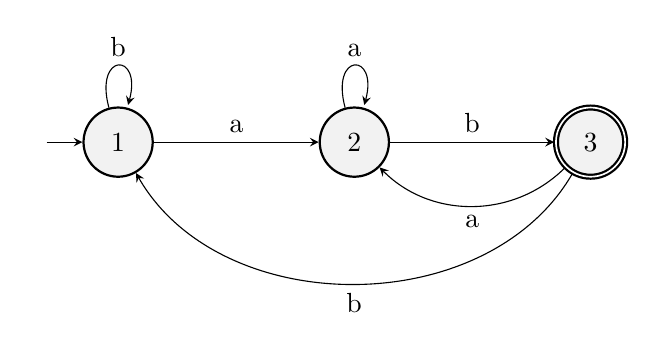
\begin{tikzpicture}
    \node[state, initial] (q1) {1};
    \node[state] (q2) [right of=q1] {2};
    \node[state, accepting] (q3) [right of=q2] {3};

    \path
        (q1) edge [loop above] node {b} (q1)
             edge node[above] {a} (q2)
        (q2) edge [loop above] node {a} (q2)
             edge node[above] {b} (q3)
        (q3) edge [bend left=45] node[below] {a} (q2)
             edge [bend left=60] node[below] {b} (q1);
\end{tikzpicture}
\end{center}

% ---------------------------------------------------------
\vspace{0.5cm}
\textbf{2. All the words that contain $aba$}

\begin{center}
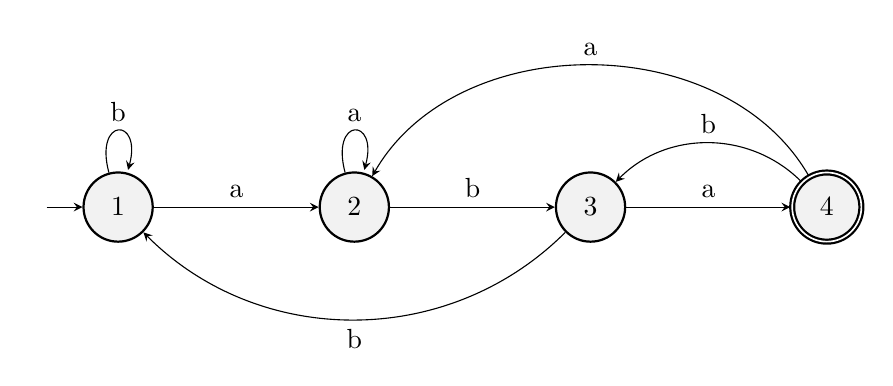
\begin{tikzpicture}
    \node[state, initial] (q1) {1};
    \node[state] (q2) [right of=q1] {2};
    \node[state] (q3) [right of=q2] {3};
    \node[state, accepting] (q4) [right of=q3] {4};

    \path
        (q1) edge [loop above] node {b} (q1)
             edge node[above] {a} (q2)
        (q2) edge [loop above] node {a} (q2)
             edge node[above] {b} (q3)
        (q3) edge [bend left=45] node[below] {b} (q1)
             edge node[above] {a} (q4)
        (q4) edge [bend right=60] node[above] {a} (q2)
             edge [bend right=45] node[above] {b} (q3);
\end{tikzpicture}
\end{center}

% ---------------------------------------------------------
\vspace{0.5cm}
\textbf{3. All the words that contain an odd number of $a$'s and an odd number of $b$'s}

\begin{center}
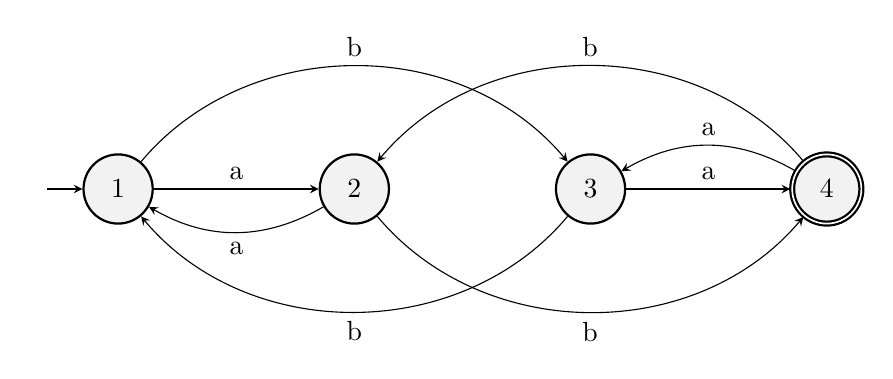
\begin{tikzpicture}
    \node[state, initial] (q1) {1};
    \node[state] (q2) [right of=q1] {2};
    \node[state] (q3) [right of=q2] {3};
    \node[state, accepting] (q4) [right of=q3] {4};

    \path
        (q1) edge node[above] {a} (q2)
             edge [bend left=50] node[above] {b} (q3)
        (q2) edge [bend left] node[below] {a} (q1)
             edge [bend right=50] node[below] {b} (q4)
        (q3) edge [bend left=50] node[below] {b} (q1)
             edge node[above] {a} (q4)
        (q4) edge [bend right=50] node[above] {b} (q2)
             edge [bend right] node[above] {a} (q3);
\end{tikzpicture}
\end{center}

% ---------------------------------------------------------
\vspace{0.5cm}
\textbf{4. All the words that contain an even number of $a$'s and an odd number of $b$'s}

\begin{center}
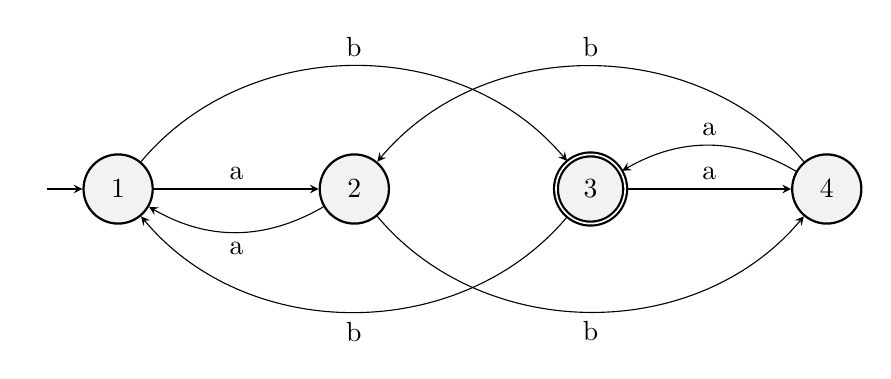
\begin{tikzpicture}
    \node[state, initial] (q1) {1};
    \node[state] (q2) [right of=q1] {2};
    \node[state, accepting] (q3) [right of=q2] {3};
    \node[state] (q4) [right of=q3] {4};

    \path
        (q1) edge node[above] {a} (q2)
             edge [bend left=50] node[above] {b} (q3)
        (q2) edge [bend left] node[below] {a} (q1)
             edge [bend right=50] node[below] {b} (q4)
        (q3) edge [bend left=50] node[below] {b} (q1)
             edge node[above] {a} (q4)
        (q4) edge [bend right=50] node[above] {b} (q2)
             edge [bend right] node[above] {a} (q3);
\end{tikzpicture}
\end{center}

% ---------------------------------------------------------
\vspace{0.5cm}
\textbf{5. All the words such that any three consecutive characters contain at least one $a$}

\begin{center}
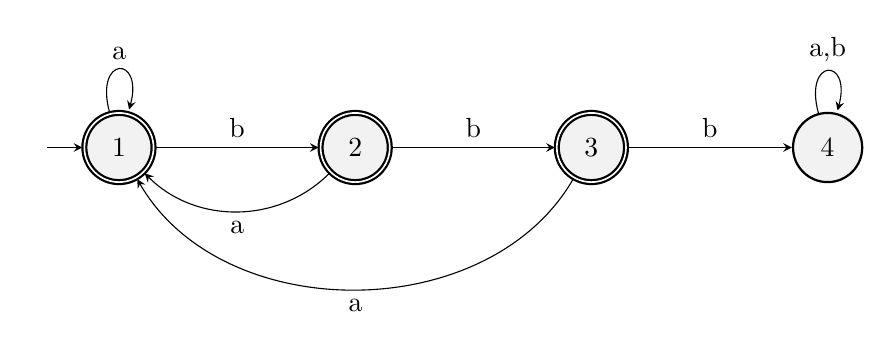
\begin{tikzpicture}
    \node[state, initial, accepting] (q1) {1};
    \node[state, accepting] (q2) [right of=q1] {2};
    \node[state, accepting] (q3) [right of=q2] {3};
    \node[state] (q4) [right of=q3] {4};

    \path
        (q1) edge [loop above] node {a} (q1)
             edge node[above] {b} (q2)
        (q2) edge [bend left=45] node[below] {a} (q1)
             edge node[above] {b} (q3)
        (q3) edge [bend left=60] node[below] {a} (q1)
             edge node[above] {b} (q4)
        (q4) edge [loop above] node {a,b} (q4);
\end{tikzpicture}
\end{center}

% ---------------------------------------------------------
\vspace{0.5cm}
\textbf{6. All the words that contain $bbb$}

\begin{center}
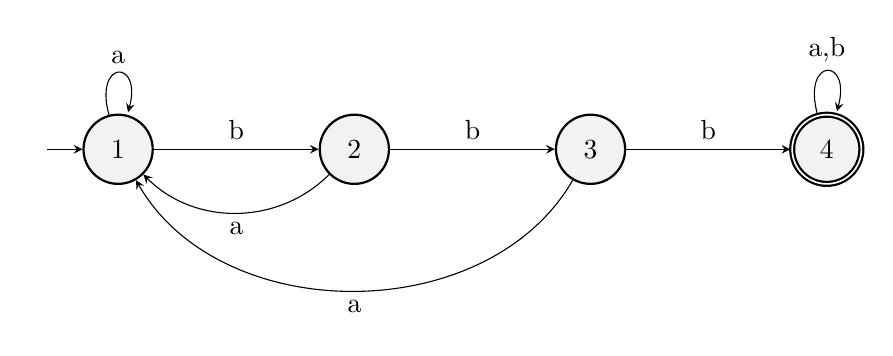
\begin{tikzpicture}
    \node[state, initial] (q1) {1};
    \node[state] (q2) [right of=q1] {2};
    \node[state] (q3) [right of=q2] {3};
    \node[state, accepting] (q4) [right of=q3] {4};

    \path
        (q1) edge [loop above] node {a} (q1)
             edge node[above] {b} (q2)
        (q2) edge [bend left=45] node[below] {a} (q1)
             edge node[above] {b} (q3)
        (q3) edge [bend left=60] node[below] {a} (q1)
             edge node[above] {b} (q4)
        (q4) edge [loop above] node {a,b} (q4);
\end{tikzpicture}
\end{center}

\textbf{What do you notice when comparing the various automata?}

For DFAs that have criteria of "ends with," arrows must leave the accept state because the string could keep going and fail to satisfy DFA characteristics. For DFAs that have criteria of , "contains," the accept state must be a "Trap State" with a self-loop, because once you find the sequence, you can traverse through the DFA while satisfying DFA's accepted language conditions.

\subsubsection{Question}
What is the easiest and best way to implement DFAs in programming?

\section{Synthesis}

\section{Evidence of Participation}

\section{Conclusion}\label{conclusion}

\begin{thebibliography}{99}
\bibitem[BLA]{bla} Author, \href{https://en.wikipedia.org/wiki/LaTeX}{Title}, Publisher, Year.
\end{thebibliography}

\end{document}
